\let\negmedspace\undefined
\let\negthickspace\undefined
\documentclass[journal]{IEEEtran}
\usepackage[a5paper, margin=10mm, onecolumn]{geometry}
%\usepackage{lmodern} % Ensure lmodern is loaded for pdflatex
\usepackage{tfrupee} % Include tfrupee package

\setlength{\headheight}{1cm} % Set the height of the header box
\setlength{\headsep}{0mm}     % Set the distance between the header box and the top of the text

\usepackage{gvv-book}
\usepackage{gvv}
\usepackage{cite}
\usepackage{amsmath,amssymb,amsfonts,amsthm}
\usepackage{algorithmic}
\usepackage{graphicx}
\usepackage{textcomp}
\usepackage{xcolor}
\usepackage{txfonts}
\usepackage{listings}
\usepackage{enumitem}
\usepackage{mathtools}
\usepackage{gensymb}
\usepackage{comment}
\usepackage[breaklinks=true]{hyperref}
\usepackage{tkz-euclide} 
\usepackage{listings}
% \usepackage{gvv}                                        
\def\inputGnumericTable{}                                 
\usepackage[latin1]{inputenc}                                
\usepackage{color}                                            
\usepackage{array}                                            
\usepackage{longtable}                                       
\usepackage{calc}                                             
\usepackage{multirow}                                         
\usepackage{hhline}                                           
\usepackage{ifthen}                                           
\usepackage{lscape}
\begin{document}

\bibliographystyle{IEEEtran}

\title{4.13.28}
\author{EE25BTECH11023 - Venkata Sai}
% \maketitle
% \newpage
% \bigskip
\maketitle \vspace{-1cm}
\renewcommand{\thefigure}{\theenumi}
\renewcommand{\thetable}{\theenumi}
\setlength{\intextsep}{10pt} % Space between text and floats

\numberwithin{align}{enumi}
\numberwithin{figure}{enumi}
\renewcommand{\thetable}{\theenumi}

\textbf{Question:}  \\
Slope of a line passing through $\vec{P}\brak{2,3}$ and intersecting the line $x+y=7$ at a distance of 4 units from $\vec{P}$, is

\textbf{Solution:}  
Given  
\begin{align}
\vec{P}=\myvec{2\\3}
\end{align}
Equation of a line through $\vec{P}$ and having slope $m$ is
\begin{align}
\vec{r}=\vec{p}+t\vec{b} \\
\vec{b}=\myvec{1\\m}
 \end{align}
\begin{align}
  x+y=7 \implies  \myvec{1 & 1}\vec{x}=7 \\
  \myvec{1&1}\brak{\vec{p}+t\vec{b}}=7
\end{align}
\begin{align}
\myvec{1&1}\vec{p}+t\myvec{1&1}\vec{b} = 7\\
t\myvec{1&1}\vec{b} =7-\myvec{1&1}\vec{p} \\
t=\frac{7-\myvec{1&1}\vec{p}}{\myvec{1&1}\vec{b}}
\end{align}
$\vec{Q}$ be the point of intersection
\begin{align}
\vec{q}=\vec{p}+t\vec{b} \\
\vec{q}-\vec{p}=t\vec{b} 
\end{align}
\begin{align}
\norm{\vec{q}-\vec{p}}=|t|\norm{\vec{b}} 
\implies |t|=\frac{\norm{\vec{q}-\vec{p}}}{\norm{\vec{b}}} 
\end{align}
\begin{align}
\left|  \frac{7-\myvec{1&1}\vec{p}}{\myvec{1&1}\vec{b}} \right|=\frac{\norm{\vec{q}-\vec{p}}}{\norm{\vec{b}}}
\end{align}
Given the point is at a distance of 4 units from point $\vec{P}$
\begin{align}
 \left|  \frac{7-\myvec{1&1}\myvec{2\\3}}{\myvec{1&1}\myvec{1\\m}} \right| =\frac{4}{\sqrt{1+m^2}} 
\end{align}
\begin{align}
\left|\frac{7-5}{1+m}\right|&=\frac{4}{\sqrt{1+m^2}} \\
\brak{\frac{7-5}{1+m}}^2=\frac{16}{1+m^2} &\implies \frac{4}{\brak{1+m}^2}=\frac{16}{1+m^2} \\
4\brak{1+m}^2&=1+m^2 
\end{align}
\begin{align}
4\brak{m^2+2m+1}=1+m^2 
\end{align}
\begin{align}
4m^2+8m+4=1+m^2 &\implies 3m^2 + 8m + 3 = 0 \\
m^2 +\frac{8m}{3}& + 1 = 0 \\
m^2 +\frac{8m}{3} + 1 &+\brak{\frac{4}{3}}^2= \frac{16}{9} \\
\brak{m+\frac{4}{3}}^2=&\frac{16-9}{9}=\frac{7}{9} \\
m+\frac{4}{3}&=\pm\frac{\sqrt{7}}{3}
\end{align}
\begin{align}  
m=\frac{-4-\sqrt{7}}{3}\ \brak{\text{or}}\ \frac{-4+\sqrt{7}}{3}
\end{align}
According to options
\begin{align}
m=\frac{-4+\sqrt{7}}{3}=\frac{8-2\sqrt{7}}{-6}=\frac{\brak{1-\sqrt{7}}^2}{\brak{1+\sqrt{7}}\brak{1-\sqrt{7}}}=\frac{1-\sqrt{7}}{1+\sqrt{7}}
\end{align}
\begin{figure}[h!]
   \centering
   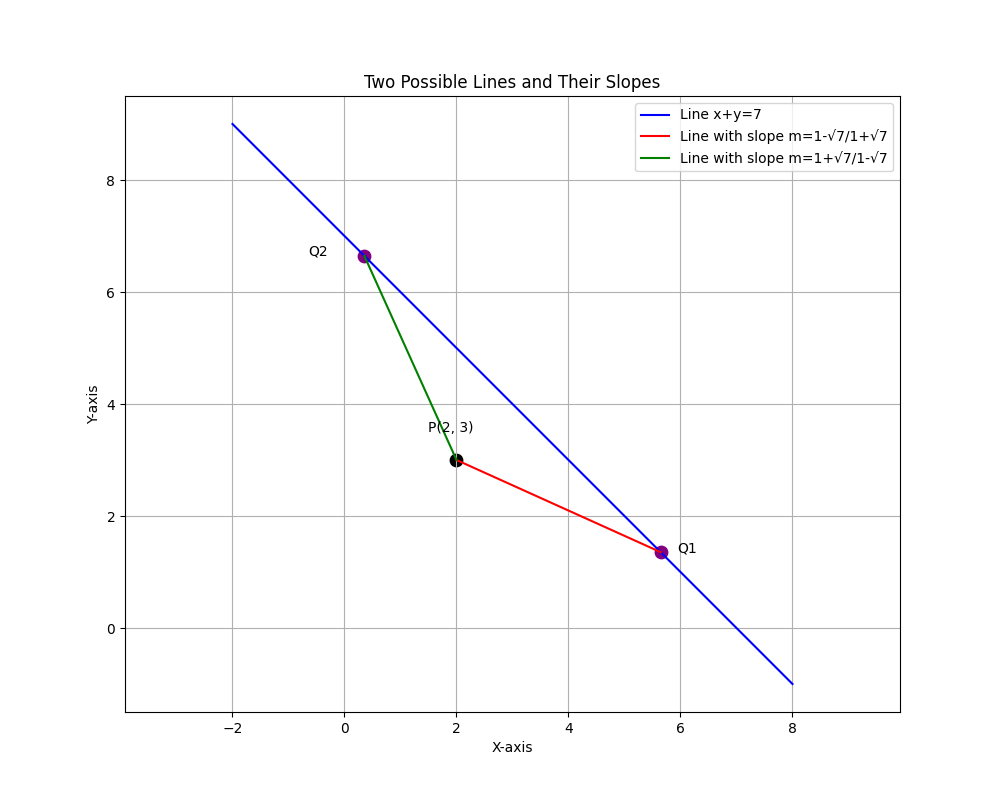
\includegraphics[width=0.6\columnwidth]{figs/fig1.png}
   \caption{}
   \label{Figure}
\end{figure}
\end{document}  
